\documentclass[../../main.tex]{subfiles}

\begin{document}

    \subsection{Scenarios}

      \newcounter{ScenarioCounter}
      
      \stepcounter{ScenarioCounter}
      \subsubsection{Scenario \arabic{ScenarioCounter}}

        Luca lives in a country where lockdown policies are applied. The last time he shopped for groceries online, 
        he forgot to add to the cart olive oil, and now he needs it. Waiting until the next delivery would take too much time, 
        so Luca decides to line up for the nearest store. 
        Luca opens CLup, looks for the nearest store and selects it. 
        He then inserts the expected duration of his visit and the category of the item he wants to buy. 
        Unfortunately, CLup estimates that the olive oil department will be busy for the next hours. 
        CLup suggests an alternative store in proximity, where there is a free slot sooner. 
        Luca accepts the suggestion and CLup queues Luca to access the store. Luca receives confirmation.

      \stepcounter{ScenarioCounter}
      \subsubsection{Scenario \arabic{ScenarioCounter}}

        Anna, a long time customer of the local store, wants to reserve a time slot to go grocery shopping the next week. 
        Anna opens CLup and selects the desired store and the desired date and time slot. 
        Not knowing yet which articles she might need, she does not fill the product categories section, 
        and she does not provide any visit duration estimation. Once Anna confirms her intentions to CLup, 
        the system predicts automatically the duration and the departments she is most likely to be in, 
        based on the collected history of previous visits. CLup then checks if Anna's visit is compatible with the 
        current schedule of the store, and, as the answer is positive, it shows a confirmation of the reservation to Anna.

      \stepcounter{ScenarioCounter}
      \subsubsection{Scenario \arabic{ScenarioCounter}}

        Maurizio reserved a slot in the queue to access the nearby store through CLup, but, due to an unforeseen commitment, 
        he has to cancel the appointment. Maurizio opens CLup, selects the reservation and cancels it. 
        The system removes Maurizio from the queue and sends a confirmation to the customer. 
        Meanwhile, Patrizia wanted to access the store as soon as possible, but all the nearest time slots were busy, 
        and the system delayed her reservation. CLup, aware of the recently freed time slot, sends a notification to Patrizia offering her to take it over. 
        Patrizia opens CLup, accepts the offering and CLup queues her in the time slot.


      \stepcounter{ScenarioCounter}
      \subsubsection{Scenario \arabic{ScenarioCounter}}

        Alina is in line through CLup to access a store and her visit start time is near. 
        CLup sends a notification to Alina to remind her of the visit. 
        Alina departs from her home and approaches the store, showing the receipt on her IT device to the receipt scanner. 
        CLup checks if the customer arrived either too early or too late with respect to the assigned time slot. 
        Alina is perfectly in time and is allowed to enter the store. Finally, when the visit is coming to an end, 
        Alina's receipt is shown once again at the store cashier, who scans it. 
        CLup registers the end of the visit and sends a confirmation message to the cashier.


      \stepcounter{ScenarioCounter}
      \subsubsection{Scenario \arabic{ScenarioCounter}}

        Alessandro, a nurse, would like to stop at the store on the way home from work to do some urgent grocery shopping. 
        Unfortunately, Alessandro's smartphone is out of charge, and he cannot use CLup's application. 
        Alessandro stops at the store anyway, approaches the store assistant at the entrance, and asks for a receipt. 
        The store assistant accesses CLup and requests to queue a visitor. The system adds the customer to the queue and sends the line up receipt as a confirmation. 
        The store assistant prints the line up receipt and gives it to Alessandro, who waits his turn.



      \stepcounter{ScenarioCounter}
      \subsubsection{Scenario \arabic{ScenarioCounter}}

        Andrea does not own either a smartphone or a personal computer. 
        Andrea would want to queue up immediately to go grocery shopping in a store adopting the CLup system, 
        but, as he is missing any IT device, he can not access the system through the Internet. 
        Andrea calls CLup's number, and the system guides him through the process: first of all, 
        the synthesized voice asks Andrea if he would like to access the store as soon as possible or to reserve a time slot, 
        and then the store he would like to visit. Once Andrea has answered the questions and confirmed his intentions, 
        the system adds Andrea to the queue of the store. The system then dictates the numeric code to be used at the entrance of the store. 
        Once Andrea confirms that he has understood the code, the interaction is closed.



      \stepcounter{ScenarioCounter}
      \subsubsection{Scenario \arabic{ScenarioCounter}}

        This time, Andrea would want to reserve a time slot to go grocery shopping next week. 
        Andrea calls CLup's number and states, once asked, that he would like to use the reservation functionalities. 
        CLup asks Andrea, in sequence, which store he would like to access, at what date, and at which time. 
        The system repeats Andrea's choices and asks for confirmation. Once Andrea confirms, 
        the system estimates the visit duration and checks if it is compatible with the current schedule. 
        The system then dictates the numeric code to be used at the entrance of the store. 
        Once Andrea confirms that he has understood the code, the interaction is closed.

        The following week Andrea gets a call from CLup, as a notification for the incoming visit. 
        As Andrea approaches the store, he goes to the store assistant, and shows her the numeric code 
        for the visit.
        The store assistant accesses CLup, and provides the system the numeric code. 
        The system gives a successful response to the store assistant, who then prints the ticket valid 
        for the visit and hands it to Andrea. 
        Now Andrea can access the store and do the shopping.



      \stepcounter{ScenarioCounter}
      \subsubsection{Scenario \arabic{ScenarioCounter}}

        Michael is a store manager at a famous supermarket chain, in a country in which COVID 
        restrictions are in effects.
        One day, the country's government releases new safety standards for supermarkets safety, which 
        includes the maximum amount of people per squared meter who can access the store. 
        The next day, before the store opening, Michael needs to update its safety parameters with the 
        newly defined ones. 
        To do this, Michael accesses CLup system, and then requests to update the safety parameters. 
        The system asks Michael for the confirmation and he confirms. 
        The system now saves the new parameters, and puts them into effect, modifying the store queue 
        availability.



      \stepcounter{ScenarioCounter}
      \subsubsection{Scenario \arabic{ScenarioCounter}}

        The same day Michael set the new safety parameters, the authorities come into his supermarket, 
        asking for the supermarket's statistics about customers flux inside the supermarket. 
        Michael accesses CLup system, and then requests to see the required statistics. 
        The system provides the requested statistics, and Michael hands them to the authorities. 



    \subsection{Use cases and sequence diagrams}

      \begin{figure}[H]
        \centering
        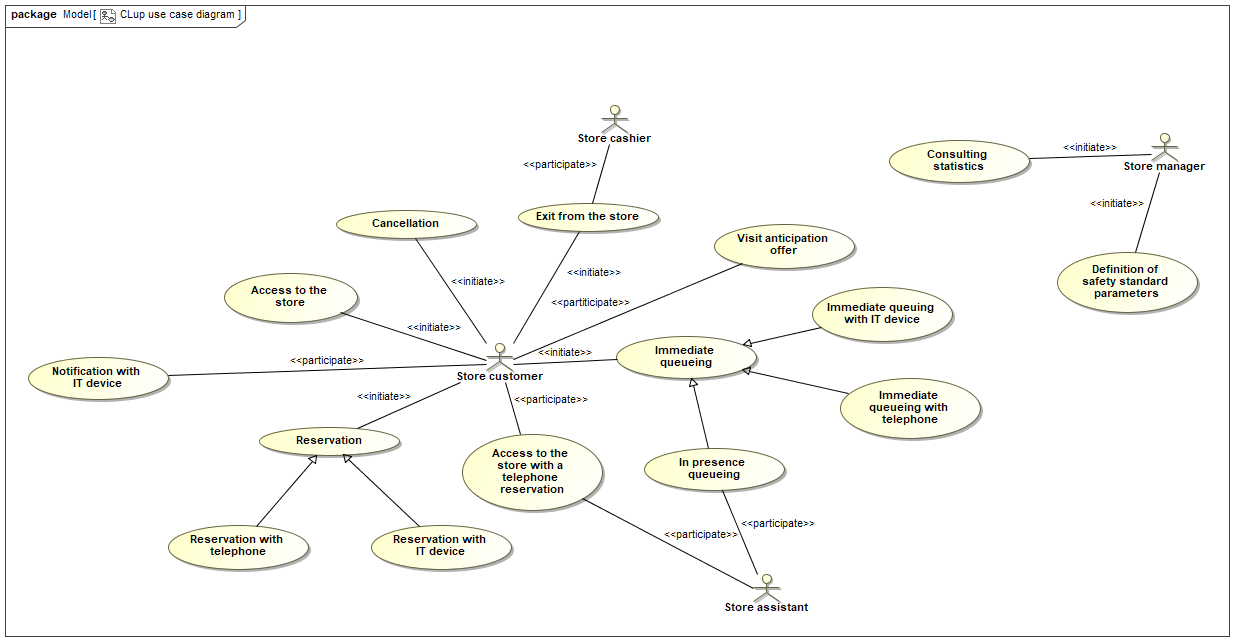
\includegraphics[width=\textwidth]{CLup_use_case_diagram.png}
        \caption{Use case diagram}
      \end{figure}

      \subsubsection{Immediate queueing with IT device}

      \begin{table}[H]
        \centering
          \begin{tabular}{c m{.75\textwidth}}
          \hline
          \textbf{Use Case} & Immediate queueing with IT device\\ \hline
          \textbf{Actor} & Store's customer\\ \hline
          \textbf{Entry condition} & The customer wants to access a store as soon as possible\\  \hline
          \textbf{Flow of events} & \begin{itemize}
                                      \item The customer selects the store they want to access
                                      \item The customer inserts the expected duration of the visit
                                      \item The customer inserts the categories of products they want to buy
                                      \item The customer confirms their intention
                                      \item The system estimates the expected duration of the visit and the visited departments
                                      \item The system checks if the store has a free slot for the customer
                                      \item The store has a free slot
                                      \item The system queues the customer
                                    \end{itemize}\\ \hline
          \textbf{Exit condition} & The system shows a confirmation message to the user \\ \hline
          \textbf{Exceptions} &  If the store does not currently have a free time slot, the system will suggest an alternative store.
                                  
                                If the customer still wants to queue for their store of choice, the system queues the user for the first available time slot. \\ \hline
          \textbf{Special requirements} &\\ \hline
          \end{tabular}
      \end{table}

      \begin{figure}[H]
        \centering
        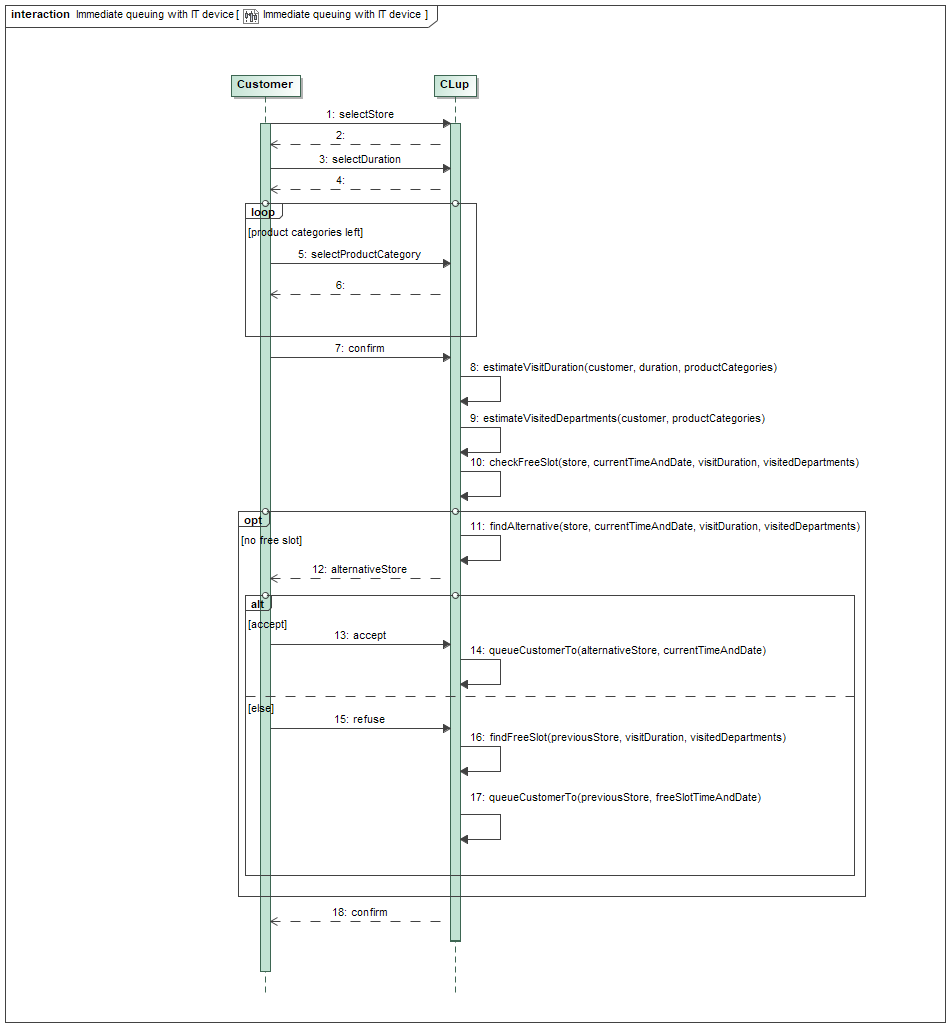
\includegraphics[width=\textwidth]{Immediate_queueing_with_IT_device.png}
        \caption{Immediate queuing with IT device sequence diagram}
      \end{figure}

      \subsubsection{Reservation with IT device}

      \begin{table}[H]
        \centering
          \begin{tabular}{c m{.75\textwidth}}
          \hline
          \textbf{Use Case} & Reservation with IT device\\ \hline
          \textbf{Actor} & Store's customer\\ \hline
          \textbf{Entry condition} & The customer wants to reserve a visit to the store\\  \hline
          \textbf{Flow of events} & \begin{itemize}
                                      \item The customer selects the store they want to access
                                      \item The customer selects the time and date of the visit
                                      \item The customer confirms their intention
                                      \item The system estimates the expected duration of the visit and the visited departments
                                      \item The system checks if the store has a free slot for the customer
                                      \item The store has a free slot
                                      \item The system queues the customer in the time slot
                                    \end{itemize}\\ \hline
          \textbf{Exit condition} & The system shows a confirmation message to the user \\ \hline
          \textbf{Exceptions} & If the desired time slot and store are not compatible with the current scheduled queue, the system will suggest an alternative. \\ \hline
          \textbf{Special requirements} &\\ \hline
          \end{tabular}
      \end{table}

      \begin{figure}[H]
        \centering
        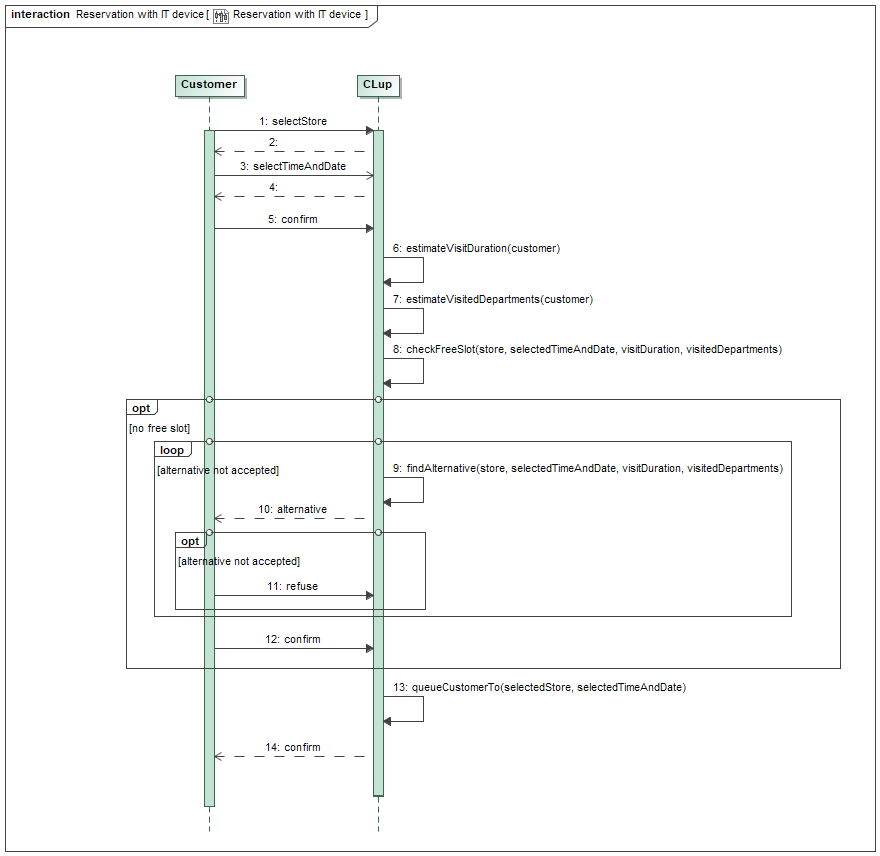
\includegraphics[width=\textwidth]{Reservation_with_IT_device.png}
        \caption{Reservation with IT device sequence diagram}
      \end{figure}


      \subsubsection{Cancellation}

      \begin{table}[H]
        \centering
          \begin{tabular}{c m{.75\textwidth}}
          \hline
          \textbf{Use Case} & Cancellation\\ \hline
          \textbf{Actor} & Store's customer\\ \hline
          \textbf{Entry condition} & A customer wants to cancel their reservation\\  \hline
          \textbf{Flow of events} & \begin{itemize}
                                      \item The customer select the cancellation option
                                      \item CLup removes the customer from the queue
                                    \end{itemize}\\ \hline
          \textbf{Exit condition} & The system shows a confirmation message to the user \\ \hline
          \textbf{Exceptions} &\\ \hline
          \textbf{Special requirements} &\\ \hline
          \end{tabular}
      \end{table}

      \begin{figure}[H]
        \centering
        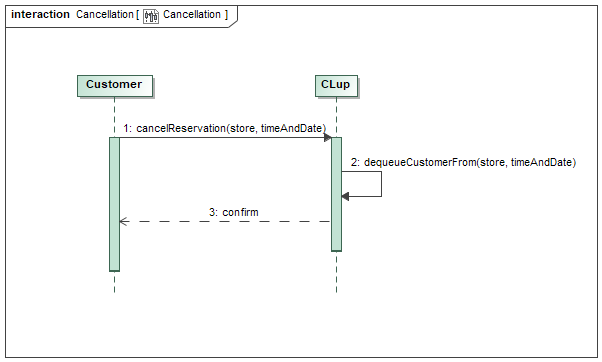
\includegraphics[width=\textwidth]{Cancellation.png}
        \caption{Cancellation sequence diagram}
      \end{figure}

      
      \subsubsection{Visit anticipation offer}

      \begin{table}[H]
        \centering
          \begin{tabular}{c m{.75\textwidth}}
          \hline
          \textbf{Use Case} & Visit anticipation offer\\ \hline
          \textbf{Actor} & Store's customer\\ \hline
          \textbf{Entry condition} & A customer cancels their reservation\\  \hline
          \textbf{Flow of events} & \begin{itemize}
                                      \item CLup checks if there is some user wanting to access the store as soon as possible and scheduled for a later visit
                                      \item CLup sends a notification to the customer, offering to move up the visit
                                      \item The customer accepts the offer
                                      \item CLup queues the customer in the time slot
                                    \end{itemize}\\ \hline
          \textbf{Exit condition} & The system shows a confirmation message to the user \\ \hline
          \textbf{Exceptions} & If no user accepts, the slot is kept free. \\ \hline
          \textbf{Special requirements} &\\ \hline
          \end{tabular}
      \end{table}

      \begin{figure}[H]
        \centering
        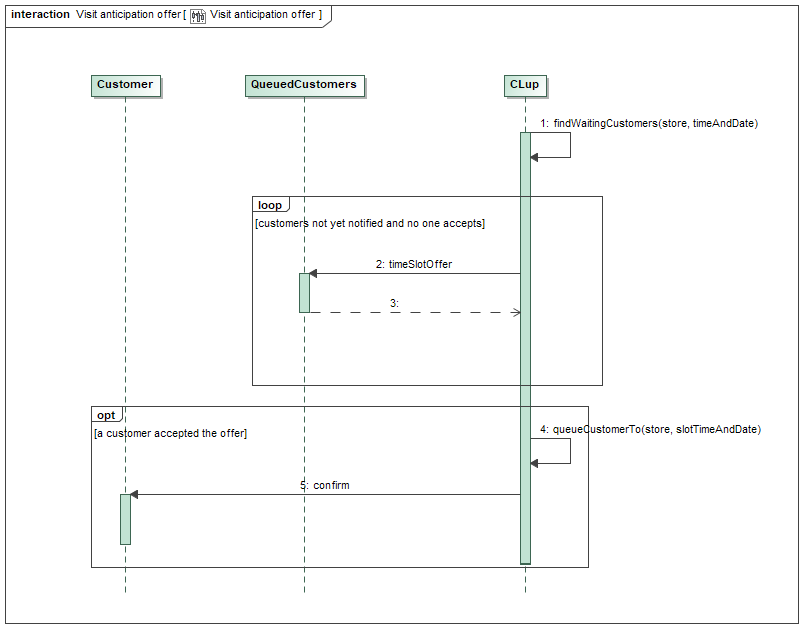
\includegraphics[width=\textwidth]{Visit_anticipation_offer.png}
        \caption{Visit anticipation offer sequence diagram}
      \end{figure}


      \subsubsection{Notification with IT device}

      \begin{table}[H]
        \centering
          \begin{tabular}{c m{.75\textwidth}}
          \hline
          \textbf{Use Case} & Notification with IT device \\ \hline
          \textbf{Actor} & Store's customer\\ \hline
          \textbf{Entry condition} & A customer's visit start time is near\\  \hline
          \textbf{Flow of events} & \begin{itemize}
                                      \item CLup sends the customer a notification to remind them of the visit
                                    \end{itemize}\\ \hline
          \textbf{Exit condition} & The customer approaches the store \\ \hline
          \textbf{Exceptions} & \\ \hline
          \textbf{Special requirements} &\\ \hline
          \end{tabular}
      \end{table}

      \begin{figure}[H]
        \centering
        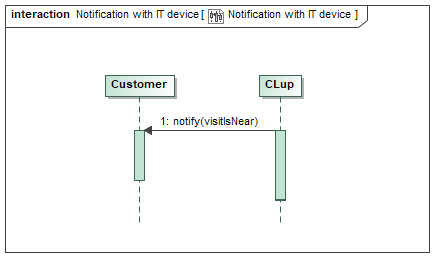
\includegraphics[width=\textwidth]{Notification_with_IT_device.png}
        \caption{Notification with IT device sequence diagram}
      \end{figure}


      \subsubsection{Access to the store}

      \begin{table}[H]
        \centering
          \begin{tabular}{c m{.75\textwidth}}
          \hline
          \textbf{Use Case} & Access to the store \\ \hline
          \textbf{Actor} & Store's customer\\ \hline
          \textbf{Entry condition} & A customer approaches the store\\  \hline
          \textbf{Flow of events} & \begin{itemize}
                                      \item The customer scans their receipt at the store entrance
                                      \item CLup checks if the current time is part of the receipt's time slot
                                    \end{itemize}\\ \hline
          \textbf{Exit condition} & CLup allows the customer to enter the store \\ \hline
          \textbf{Exceptions} & If the customer scans the receipt outside their time slot, they are not allowed to enter the store. \\ \hline
          \textbf{Special requirements} &\\ \hline
          \end{tabular}
      \end{table}

      \begin{figure}[H]
        \centering
        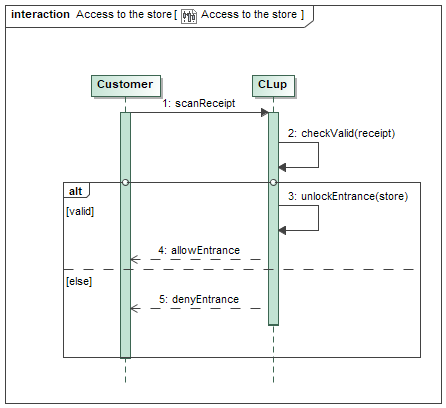
\includegraphics[width=\textwidth]{Access_to_the_store.png}
        \caption{Access to the store sequence diagram}
      \end{figure}


      \subsubsection{Exit from the store}

      \begin{table}[H]
        \centering
          \begin{tabular}{c m{.75\textwidth}}
          \hline
          \textbf{Use Case} & Exit from the store\\ \hline
          \textbf{Actor} & Store's customer, store's cashier\\ \hline
          \textbf{Entry condition} & A customer has finished shopping\\  \hline
          \textbf{Flow of events} & \begin{itemize}
                                      \item The customer shows CLup's receipt to the store's cashier
                                      \item The store's cashier scans the receipt
                                      \item CLup registers the end of the visit
                                    \end{itemize}\\ \hline
          \textbf{Exit condition} & The system shows a confirmation message to the store's cashier \\ \hline
          \textbf{Exceptions} & \\ \hline
          \textbf{Special requirements} &\\ \hline
          \end{tabular}
      \end{table}

      \begin{figure}[H]
        \centering
        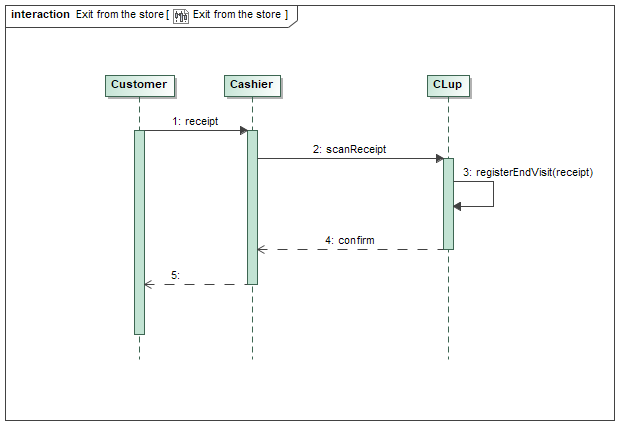
\includegraphics[width=\textwidth]{Exit_from_the_store.png}
        \caption{Exit from the store sequence diagram}
      \end{figure}


      \subsubsection{In presence queueing}

      \begin{table}[H]
        \centering
          \begin{tabular}{c m{.75\textwidth}}
          \hline
          \textbf{Use Case} & In presence queueing\\ \hline
          \textbf{Actor} & Store's customer, store assistant\\ \hline
          \textbf{Entry condition} & A customer asks a store assistant for a line up receipt\\  \hline
          \textbf{Flow of events} & \begin{itemize}
                                      \item The store assistant accesses CLup
                                      \item The store assistant requests CLup to queue the customer
                                      \item The system estimates the expected duration of the visit and the visited departments
                                      \item The system finds the first available time slot in the assistant's store
                                      \item CLup adds the customer to the queue in the first available time slot
                                      \item CLup sends the line up receipt to the store assistant as a confirmation
                                      \item The store assistant prints the line up receipt 
                                    \end{itemize}\\ \hline
          \textbf{Exit condition} & The store assistant gives the printed line up receipt to the customer\\ \hline
          \textbf{Exceptions} & \\ \hline
          \textbf{Special requirements} &\\ \hline
          \end{tabular}
      \end{table}

      \begin{figure}[H]
        \centering
        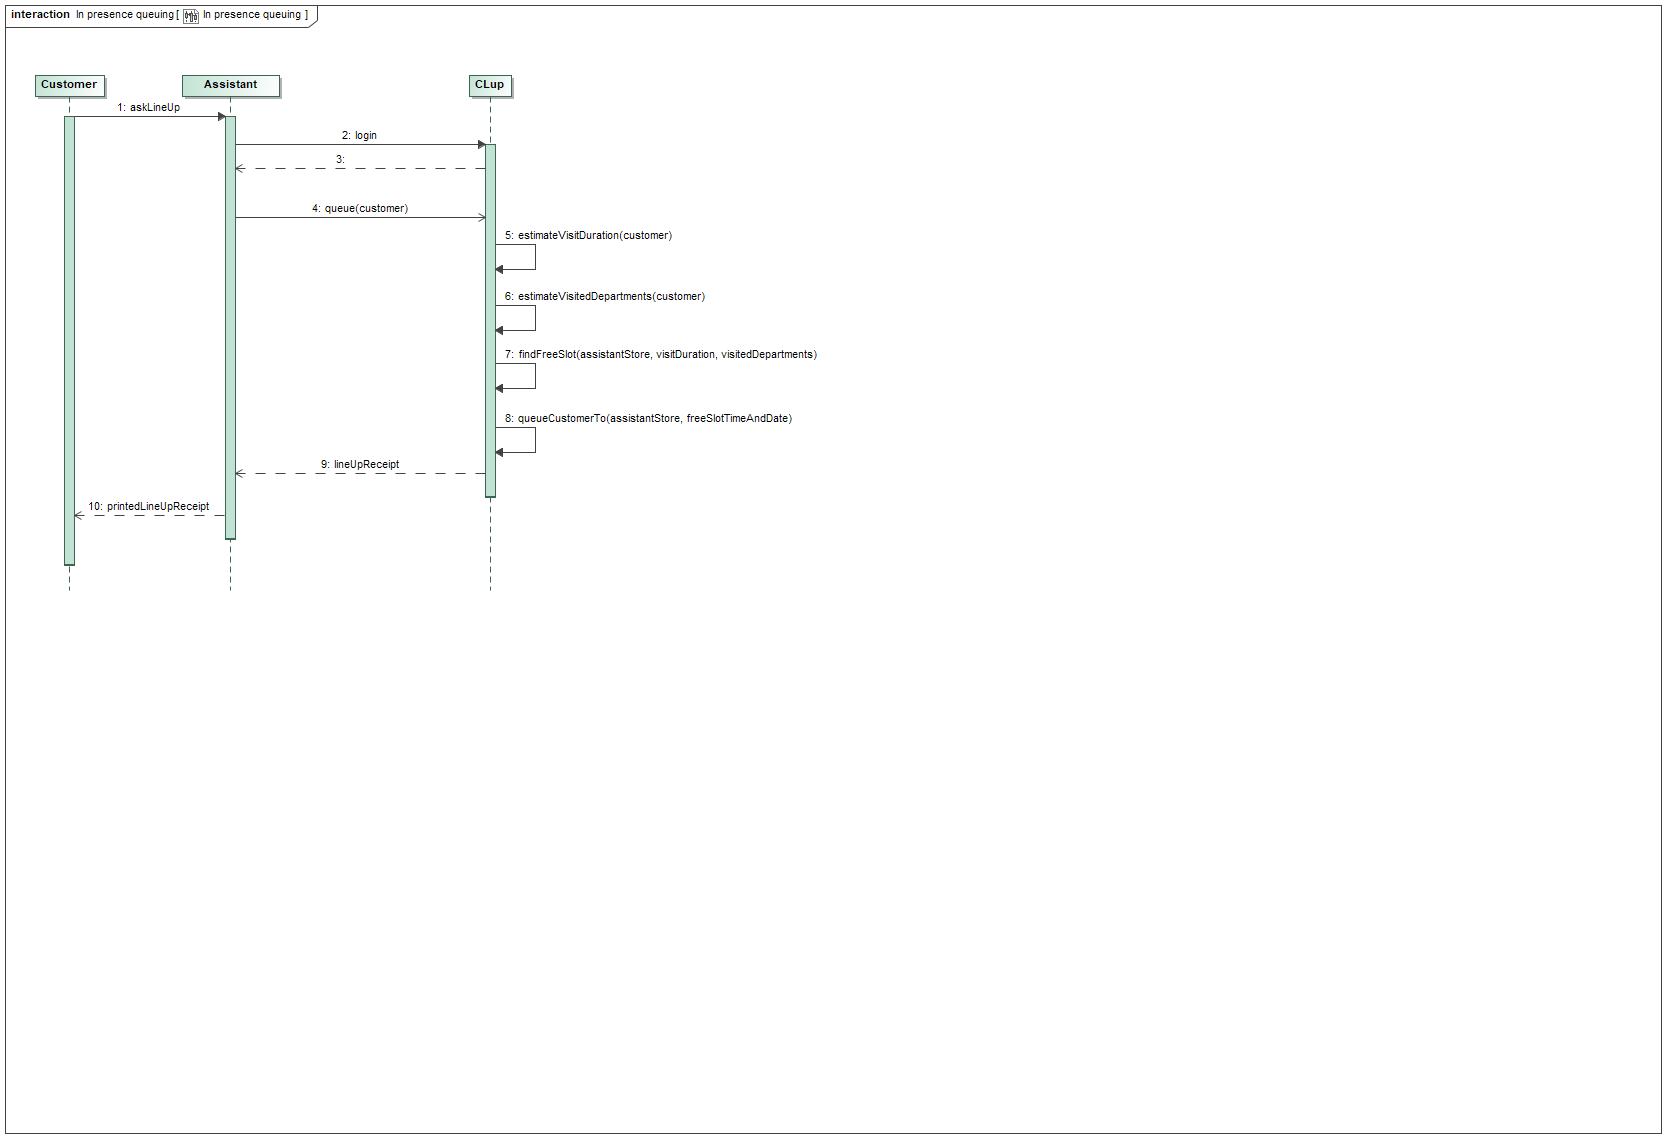
\includegraphics[width=\textwidth]{In_presence_queueing.png}
        \caption{In presence queueing sequence diagram}
      \end{figure}


      \subsubsection{Immediate queueing with telephone}

      \begin{table}[H]
        \centering
          \begin{tabular}{c m{.75\textwidth}}
          \hline
          \textbf{Use Case} & Queueing with telephone\\ \hline
          \textbf{Actor} & Store's customer\\ \hline
          \textbf{Entry condition} & A customer calls CLup's telephone number\\  \hline
          \textbf{Flow of events} & \begin{itemize}
                                      \item CLup asks the customer if they would like to access the store as soon as possible or to reserve a time slot
                                      \item The customer says they want to access the store as soon as possible
                                      \item CLup asks which store the customer wants to access
                                      \item The customer states the store they would like to access
                                      \item CLup repeats the chosen options and asks for confirmation
                                      \item The customer confirms their intentions
                                      \item The system adds the customer to the queue to enter the store
                                      \item CLup dictates the numeric code to use at the entrance to the customer
                                      \item CLup asks for confirmation that the numeric code has been understood
                                    \end{itemize}\\ \hline
          \textbf{Exit condition} & The customer confirms \\ \hline
          \textbf{Exceptions} & If the chosen store does not have any available slot, the system suggests an alternative.
          
                                If the customer does not confirm their intentions, the system states again the available options.
                                
                                If the customer does not confirm the reception of the numeric code, the system repeats the numeric code.\\ \hline
          \textbf{Special requirements} &\\ \hline
          \end{tabular}
      \end{table}

      \begin{figure}[H]
        \centering
        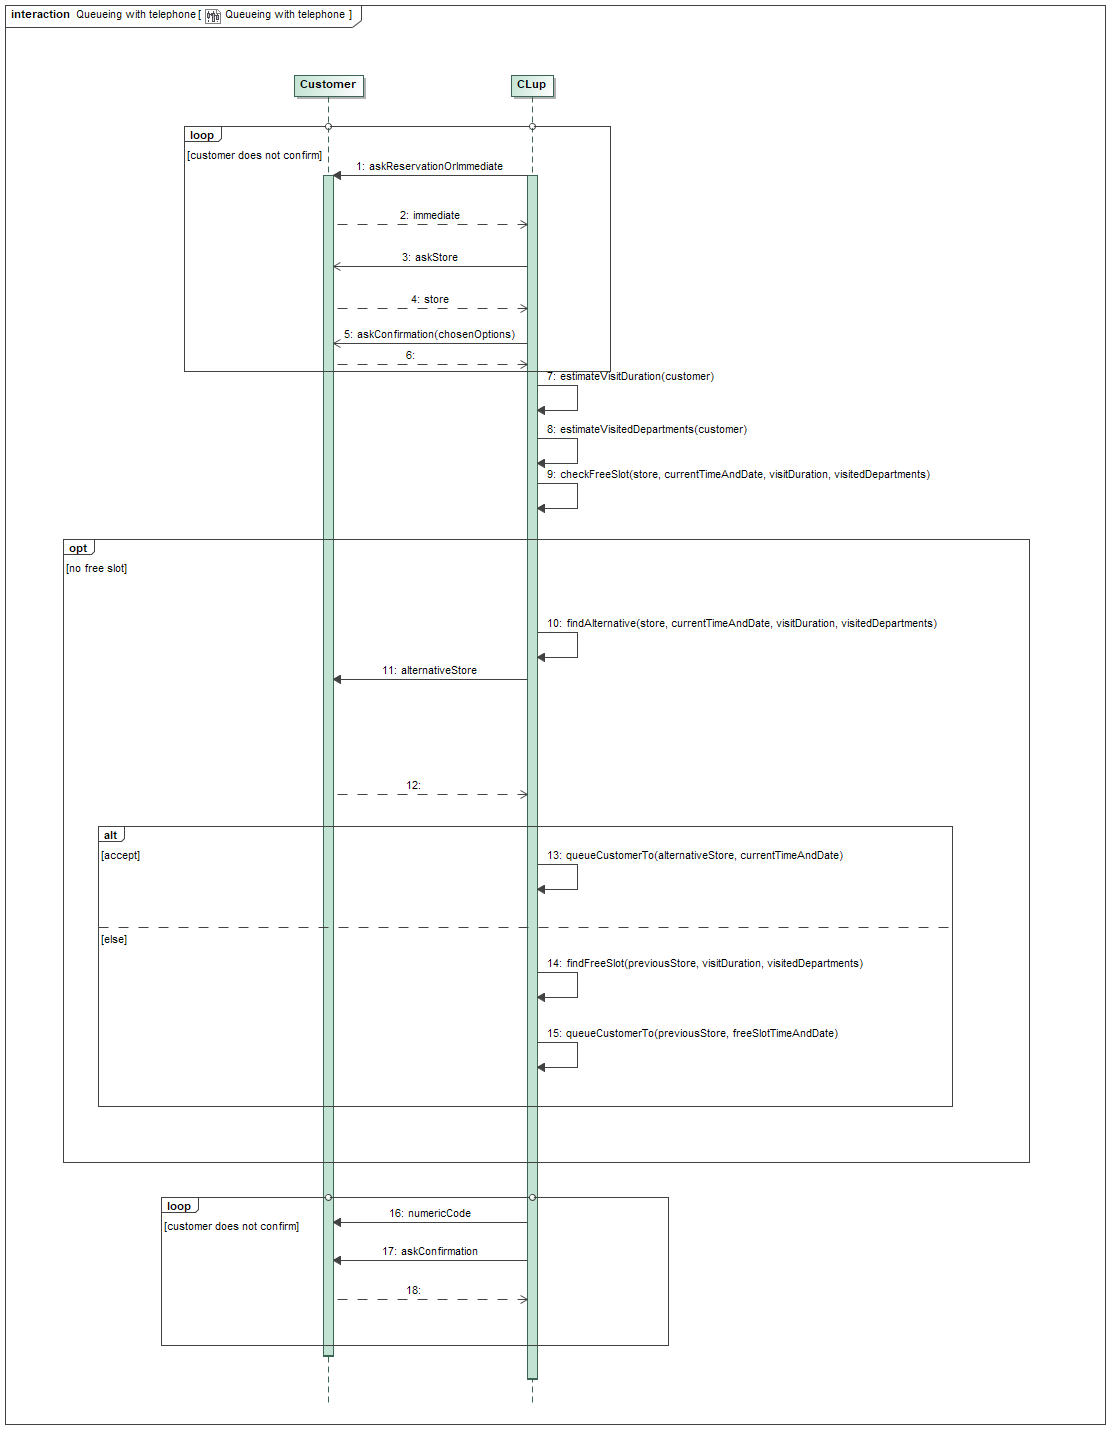
\includegraphics[width=\textwidth]{Queueing_with_telephone.png}
        \caption{Queueing with telephone sequence diagram}
      \end{figure}


      \subsubsection{Reservation with telephone}

      \begin{table}[H]
        \centering
          \begin{tabular}{c m{.75\textwidth}}
          \hline
          \textbf{Use Case} & Reservation with telephone\\ \hline
          \textbf{Actor} & Store's customer\\ \hline
          \textbf{Entry condition} & A customer calls CLup's telephone number\\  \hline
          \textbf{Flow of events} & \begin{itemize}
                                      \item CLup asks the customer if they would like to access the store as soon as possible or to reserve a time slot
                                      \item The customer says they want to reserve a time slot
                                      \item CLup asks which store the customer wants to access
                                      \item The customer states the store they would like to access
                                      \item CLup asks in which date the customer would like to access the store
                                      \item The customer states the desired date
                                      \item CLup asks at which time the customer would like to access the store
                                      \item The customer states the desired time
                                      \item CLup repeats the chosen options and asks for confirmation
                                      \item The customer confirms their intentions
                                      \item CLup estimates the visit duration
                                      \item CLup checks if the visit is compatible with the current schedule
                                      \item The system adds the customer to the queue to enter the store
                                      \item CLup dictates the numeric code to use at the entrance to the customer
                                      \item CLup asks for confirmation that the numeric code has been understood
                                    \end{itemize}\\ \hline
          \textbf{Exit condition} & The customer confirms \\ \hline
          \textbf{Exceptions} & If the reservation is not compatible with the current schedule, the system suggests an alternative.
          
                                If the customer does not confirm their intentions, the system states again the available options.
                                
                                If the customer does not confirm the reception of the numeric code, the system repeats the numeric code.\\ \hline
          \textbf{Special requirements} &\\ \hline
          \end{tabular}
      \end{table}

      \begin{figure}[H]
        \centering
        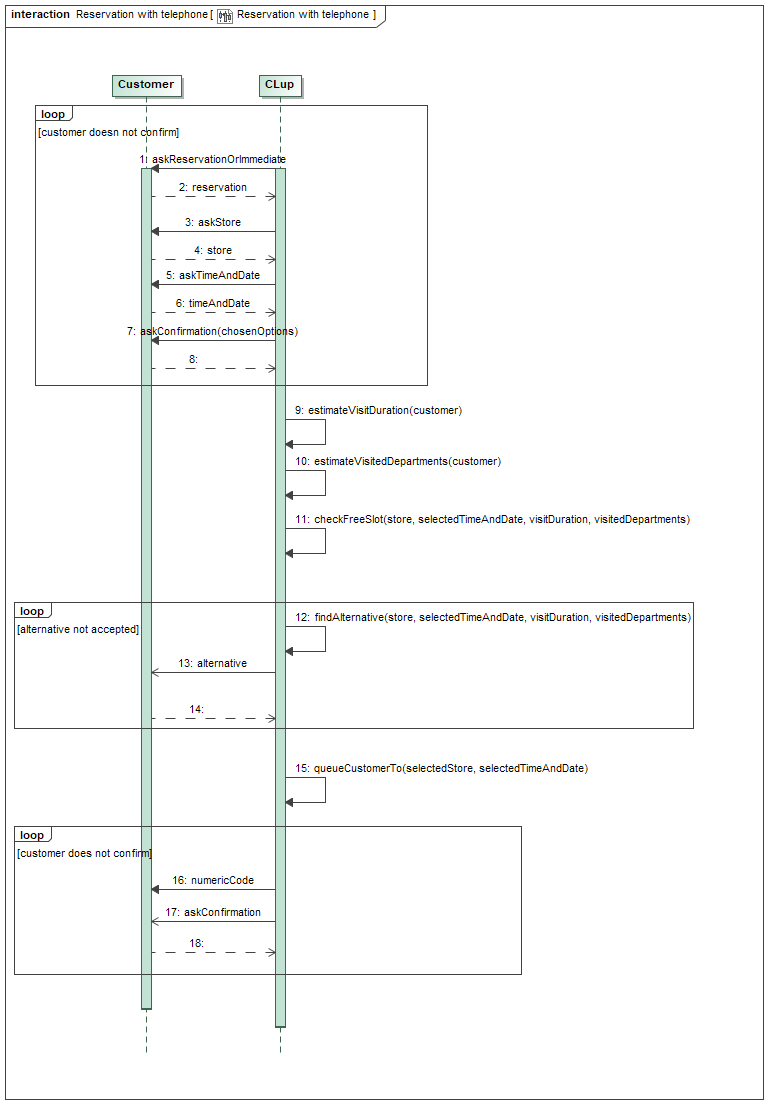
\includegraphics[width=\textwidth]{Reservation_with_telephone.png}
        \caption{Reservation with telephone sequence diagram}
      \end{figure}

      \subsubsection{Access to the store with a telephone reservation}

      \begin{table}[H]
        \centering
          \begin{tabular}{c m{.75\textwidth}}
          \hline
          \textbf{Use Case} & Accessing the store with a telephone reservation\\ \hline
          \textbf{Actor} & Store's customer, store assistant\\ \hline
          \textbf{Entry condition} & The visit start time of a customer who has reserved a place in the queue via telephone call is near\\  \hline
          \textbf{Flow of events} & \begin{itemize}
                                      \item CLup system calls the user, to remind them of the visit
                                      \item The customer approaches the store
                                      \item The customer goes to a store assistant, and shows them the numeric code
                                      \item The store assistant accesses CLup system
                                      \item The store assistant checks the numeric code
                                    \end{itemize}\\ \hline
          \textbf{Exit condition} & The store assistant prints the line up receipt \\ \hline
          \textbf{Exceptions} & If the numeric code is invalid or expired, CLup returns an error to the store assistant.\\ \hline
          \textbf{Special requirements} &\\ \hline
          \end{tabular}
      \end{table}

      %% TODO: ADD SEQUENCE DIAGRAM

      \subsubsection{Consulting statistics} %TODO

      \begin{table}[H]
        \centering
          \begin{tabular}{c m{.75\textwidth}}
          \hline
          \textbf{Use Case} & Consulting statistics\\ \hline
          \textbf{Actor} & Store manager\\ \hline
          \textbf{Entry condition} & The store manager wants to consult current statistics\\  \hline
          \textbf{Flow of events} & \begin{itemize}
                                      \item The store manager accesses CLup
                                      \item The store manager requests current statistics to CLup
                                      \item CLup computes the requested statistics
                                    \end{itemize}\\ \hline
          \textbf{Exit condition} & CLup returns the requested statistics \\ \hline
          \textbf{Exceptions} & \\ \hline
          \textbf{Special requirements} &\\ \hline
          \end{tabular}
      \end{table}

      %% TODO: ADD SEQUENCE DIAGRAM

      \subsubsection{Definition of safety standard parameters}

      \begin{table}[H]
        \centering
          \begin{tabular}{c m{.75\textwidth}}
          \hline
          \textbf{Use Case} & Definition of safety standard parameters\\ \hline
          \textbf{Actor} & Store manager\\ \hline
          \textbf{Entry condition} & The store manager needs to define or update safety parameters \\  \hline
          \textbf{Flow of events} & \begin{itemize}
                                      \item The store manager accesses CLup
                                      \item The store manager defines or updates the needed safety parameters
                                      \item CLup asks for confirmation of the new safety parameters
                                      \item The store manager confirms
                                      \item CLup saves the new safety parameters
                                      \item CLup updates the queue availability for the store according to the newly defined safety parameters
                                    \end{itemize}\\ \hline
          \textbf{Exit condition} & CLup confirms the succeeding of the operation \\ \hline
          \textbf{Exceptions} & If the store manager does not confirm, nothing happens on CLup system, and the old safety parameters are kept.\\ \hline
          \textbf{Special requirements} &\\ \hline
          \end{tabular}
      \end{table}

      %% TODO: ADD SEQUENCE DIAGRAM

    \subsection{Mapping}

    {\rowcolors{2}{white}{lightgray}
    \begin{table}[H]
      \centering
      \begin{tabular}{|l|l|}
        \hline
        \textbf{Use case} & \textbf{Requirement IDs}\\ \hline\hline
        Immediate queueing with IT device & R1, R6, R4, R8, R9, R13, R14, R15 \\
        Reservation with IT device & R1, R6, R7, R8, R9, R13, R14, R15 \\
        Cancellation & R16 \\
        Visit anticipation offer & R14, R15, R16 \\
        Notification with IT device & R10, R11 \\
        Access to the store & R10, R12 \\
        Exit from the store & R3, R12 \\
        In presence queueing & R1, R4, R5, R6, R8, R9 \\
        Immediate queueing with telephone & R1, R4, R8, R9, R13, R14, R15 \\
        Reservation with telephone & R1, R7, R8, R9, R13, R14, R15\\
        Access to the store with a telephone reservation &  R6, R10, R11\\
        Consulting statistics & R3\\
        Definition of safety standard parameters & R2\\
        \hline
      \end{tabular}
      \caption{Use case to requirements mapping}
      \end{table}
    }
    
    {\rowcolors{2}{white}{lightgray}
    \begin{table}[H]
      \centering
      \begin{tabular}{|l|l|}
        \hline
        \textbf{Goal ID} & \textbf{Requirement IDs}\\ \hline\hline
        G1 & R1, R2, R12, R13 \\
        G2 & R1, R8, R9, R13 \\
        G3 & R1, R2, R3, R8, R9, R12\\
        G4 & R4, R5, R6, R7, R10, R14, R15\\
        G5 & R7, R8, R10, R11, R16\\
        G6 & R13, R14, R15, R16\\
        G7 & R13, R14, R15, R16\\
        G8 & R7, R13, R15, R16\\
        G9 & R4, R13, R14, R16\\
        \hline
      \end{tabular}
      \caption{Goals to requirements mapping}
      \end{table}
    }
\end{document}
